\documentclass[conference]{IEEEtran}
\IEEEoverridecommandlockouts
\usepackage[a4paper]{geometry}
\geometry{verbose,tmargin=2.5cm,bmargin=2cm,lmargin=2cm,rmargin=2cm}
\usepackage{fancyhdr}
\pagestyle{fancy}

% nastavení pisma a~češtiny
\usepackage{lmodern}
\usepackage[T1]{fontenc}
\usepackage[utf8]{inputenc}
\usepackage[czech]{babel}

% odkazy
\usepackage{url}

\usepackage{float}
% vícesloupcové tabulky
\usepackage{multirow}
\usepackage{amssymb}
\usepackage{gensymb}
\usepackage{bbold}
\usepackage{mathtools}
\usepackage{commath}

% vnořené popisky obrázků
\usepackage{subcaption}

% automatická konverze EPS 
\usepackage{graphicx} 
\usepackage{epstopdf}
\usepackage{amsmath}
\usepackage{siunitx}
\usepackage{bondgraphs}
\usetikzlibrary{decorations.markings}
\epstopdfsetup{update}

% odkazy a~záložky
\usepackage[unicode=true, bookmarks=true,bookmarksnumbered=true,
bookmarksopen=false, breaklinks=false,pdfborder={0 0 0},
pdfpagemode=UseNone,backref=false,colorlinks=true] {hyperref}

% Poznámky při překladu
\usepackage{xkeyval}	% Inline todonotes
\usepackage[textsize = footnotesize]{todonotes}
\presetkeys{todonotes}{inline}{}
\graphicspath{{./images}}

%https://tex.stackexchange.com/questions/2783/bold-calligraphic-typeface
\DeclareMathAlphabet\mathbfcal{OMS}{cmsy}{b}{n}


% smaz aktualni page layout
\fancyhf{}
% zahlavi
\usepackage{titling}
\fancyhf[HC]{\thetitle}
\fancyhf[HLE,HRO]{\theauthor}
\fancyhf[HRE,HLO]{11. února 2022}
 %zapati
\fancyhf[FLE,FRO]{\thepage}

% údaje o~autorovi
\title{Modelování a~simulace dynamických systémů - semestrální úloha}
\author{Vojtěch Michal}
\date{11. února 2022}

\begin{document}

\maketitle

\section{Úvod}

Repozitář se zadáním modelovací úlohy je dostupný na školním Gitlabu ČVUT \cite{repository}, zadání samotné je dostupné na \cite{zadani}.

Laboratorní model přečerpávací vodní elektrárny sestává ze tří nádrží $\text{N}_1$ až $\text{N}_3$ propojených trubkami
s ventily a~čerpadlem. Zjednodušené schéma je na obrázku \ref{fig:schema}.

\begin{figure}[htbp]
    \centering
    \includegraphics[width=\linewidth]{vodarna_schema.eps}
    \caption{Zjednodušené schéma laboratorního modelu}
    \label{fig:schema}
\end{figure}

\section{Modelování vazebními grafy}

Instancemi \textit{zobecněného úsili} $e$ a~\textit{toku} $\dot{q}$ jsou v případě hydrodynamických systémů veličiny tlak $p$ a~objemový průtok $Q$.
Pro \textit{zobecněné poddajnosti} je důležitý integrál toku (či též \textit{zobecněné posunutí}) $\int \dot{q}~\text{d}t$,
kterým je objem $V$ vody v nádrži. Zobecněné rezistory reprezentují omezení na průtok vody trubkami a~ventily.
Místo tlaků uvažuji při řešení problému pouze přetlaky, tedy považuji atmosférický tlak $p_a$ za hladinu nulového úsilí.

\subsection{Nádrže}

Nádrž na vodu modeluje prvek zobecněná poddajnost. Protože nejsou dle zadání shora hermeticky uzavřeny, působí
na vodu atmosferický tlak, vůči kterému je vztažen hydrostatický tlak na dně nádrže. s~jeho pomocí lze odvodit modul poddajnosti.

Nechť $V$ označuje objem vody v nádrži o~výšce $h$ a~ploše podstavy $S$. Nechť $\rho$ je hustota vody
a $g$ je konstanta gravitačního zrychlení. Poté u~dna nádrže působí hydrostatický tlak
\begin{equation}
    p = h \rho g = \frac{V}{S} \rho g = V \frac{\rho g}{S}.
\end{equation}
Porovnáním s~definičním vztahem pro zobecněnou poddajnost
\begin{equation}
    e = \frac{q}{C}
\end{equation}
je zřejmé, že modul poddajnosti $i$-té nádrže je roven
\begin{equation}
    C_i = \frac{S_i}{\rho g},
    \label{eq:poddajnost}
\end{equation}
kde $S_i$ je plocha dna dané nádrže a~$\rho$ i~$g$ jsou konstanty uvedné výše.

\subsection{Trubky}

Trubky omezují tok vody po systému, je proto přirozené na ně nahlížet jako na zobecněné rezistory.
Podle \cite{odpor_trubky} platí pro odpor $i$-té trubky vůči toku kapaliny vztah
\begin{equation}
    R_{Ti} = \frac{8\eta L_i}{\pi r_i^4},
    \label{eq:odpor_trubky}
\end{equation}
kde $r_i$ a~$L_I$ jsou poloměr a~délka dané trubky a~$\eta$ je konstanta viskozity,
jež má pro vodu o~teplotě 20°C hodnotu $\eta = 1.002 \cdot 10^{-3} \si{\pascal \second}$.

Hodnota odporu $R_{T4}$ mezi spodní nádrží a~čerpadlem byla pro malou délku trubky zanedbána.
Trubka $\text{T}_1$ působí v systému odporem tak, jak vychází z rovnice \eqref{eq:odpor_trubky},
naopak odpor trubek $\text{T}_2$ a~$\text{T}_3$ je dále ovlivněn ventily na nich umístěnými.
Ventily jsou dále rozebrány v sekci \ref{sec:ventily}.

Trubky $\text{T}_1$ a~$\text{T}_3$ jsou umístěny vertikálně a~proto v nich je vlivem gravitačního působení Země různý hydrostatický
tlak v různých výškách.
U trubky $\text{T}_3$ je tento fakt zanebán, neboť v ní voda nikdy nestojí. Protože zadání garantuje, že hladina ve spodní nádrži
nikdy nedosáhne po ústí trubky $\text{T}_3$, je trubka (včetně ventilu) modelována jako prostý rezistor limitující průtok a~aktivovaná vazba
přenášející objemový průtok přímo do spodní nádrže.

\subsection{Sloupec stojící vody}
\label{sec:sloupec_vody}
Naopak trubkou $\text{T}_1$ je voda vytlačována vzhůru, jedná se tak o~homogenní sloupec vody a~u~její paty (u čerpadla)
je větší tlak než nahoře u~dna nádrže $\text{N}_1$.
Pro modelování tohoto faktu byl na spoj typu 1 reprezentující objemový průtok $Q_1$ připojen zdroj zobecněného úsilí (tlaku)
$\Delta p_{14}$ modelující úbytek vlivem působení hydrostatického tlaku. Tlakový úbytek $\Delta p_{14}$ závisí na výšce sloupce vody
v trubce, bylo by proto vhodné zavést novou zobecněnou poddajnost, jejíž stav by souvisel s~výškou vodního sloupce.
Taková struktura modelu by však byla prakticky nepříjemná kvůli interakci poddajnosti trubky a~poddajnosti nádrže nad ní umístěné.
Vystižení faktu, že nádrž se může plnit až poté, co je trubka naplněna, by vnášelo do modelu nespojitosti v okamžiku přepínání poddajností.
Vše by bylo dále komplikováno neexistencí senzoru pro výšku sloupce vody v trubce (nepozorovatelný stav) a~tedy složitostí verifikace řešení.
Pro implementaci prvního modelu bylo jednodušší použít řízený zdroj tlaku realizující funkci
\begin{equation}
    \Delta p_{14} = \begin{cases}
        0 & h_1 = 0, \\
        L_1 \rho g & h_1 \neq 0.
    \end{cases}
\end{equation}
Pro použitelnost v numerických simulacích s~konečnou přeností výpočtů byla
rovnost s~nulou $h_1 = 0$ nahrazena porovnáním $h_1 \le 10^{-4}~\si{\metre}$, což je hodnota pod rozlišovací schopností
použitého ultrazvukového senzoru výšky hladiny \cite{hladinomer}.

V modelu byla zanedbána setrvačnost vody tekoucí ve všech trubkách. Největší objem má trubka $\text{T}_1$ s~hodnotou $2.8419 \cdot 10^{-4} \si{\metre\cubed}$,
při naplnění vodou by se jednalo o~283 gramů vody. s~ohledem na fakt, že všechny děje v modelu jsou velmi pomalé (časové konstanty v řádu sekund a~více),
byly moduly setrvačnosti zanedbány.


\subsection{Ventily}
\label{sec:ventily}

Ventil $\text{V}_1$ umístěný na trubce $\text{T}_2$ je dvoustavový. Pakliže je otevřený, trubka vykazuje svůj standardní odpor $R_{T2}$.
Pakliže je uzavřený, trubkou nemůže protékat žádná voda a~odpor jde limitně do nekonečna. s~použitím dvoustavové proměnné $v_1$ definované jako
\begin{equation}
    v_1 = \begin{cases} 
        0 & \text{ventil je uzavřený}, \\
        1 & \text{ventil je otevřený},
     \end{cases}
\end{equation}
lze popsat odpor $R_2$ trubky jednoduchým vztahem
\begin{equation}
    R_2(v_1) = \frac{R_{T2}}{v_1},
    \label{eq:r2}
\end{equation}
kde dodefinovávám $\frac{x}{0} = \infty$ pro libovolné reálné $x$.

Ventil $\text{V}_2$ umístěný na trubce $\text{T}_3$ lze nastavovat spojitě na 0 až 100 \% otevření a~dále vykazuje pásmo necitlivosti
pro hdonoty otevření $\le$ 20~\%.
Nechť $v_2 \in \langle 0, 100 \rangle $ je míra otevření ventilu v procentech. Protože se jedná o~proporcionální ventil,
předpokládám popis lineární (nebo lépe řečeno afinní) funkcí. Podmínky
\begin{equation}
    \begin{split}
        R_3(v_2\le20\%) &= \infty, \\
        R_3(v_2=100\%) &= R_{T3},\\        
    \end{split}
\end{equation}
splňuje funkce
\begin{equation}
    R_3(v_2) = R_{T3} \frac{100-20}{\text{max}(v_2, 20) - 20},
    \label{eq:r3}
\end{equation}
kde opět dodefinuji $\frac{x}{0} = \infty$ pro libovolné reálné $x$.

\subsection{Čerpadlo}
Čerpadlo bylo modelováno jako prostý DC motor (systém prvního řádu) - vstupem je napětí $U_{set}$ připojené na seriové zapojení odporu $R_p$ a~indukčnosti $I_p$ vinutí
a gyrátoru, jenž přenáší výkon do hydrodynamické domény. Protože je z datasetů zřejmé, že průtok vody trubkou $\text{T}_1$ neovlivňuje
výkon čerpadla (tedy při nastaveném výkonu 0 \% maxima teče voda volně, aniž by roztáčela čerpadlo v záporném smyslu),
je vazba zřejmě pouze jednostranná. Tento fakt je modelován použitím pomocného spoje typu nula a~aktivované vazby.
Použití elektrického odporu a~indukčnosti pro popis dynamických vlastností pumpy je pohodlné,
ačkoli to nemusí přímo odpovídat podstatě funkce zařízení.


\begin{figure}[htbp]
    \centering
    \begin{tikzpicture}
        \begin{scope}[decoration={
            markings,
            mark=at position 0.5 with {\arrow[very thick]{latex}}}
            ]
            
            \node[bgelement, label=west:$p_4$] (p4) at (0,0) {0};
            \node[bgelement, label=south:$p_3$] (p3) at (4,0) {0};
            \node[bgelement, label=west:$p_1$] (p1) at (0,4) {0};
            \node[bgelement, label=east:$p_2$] (p2) at (4,4) {0};
            
            \node[bgelement, label=315:$Q_1$] (Q1_west) at (0,2) {1};
            \node[bgelement, label=east:$Q_3$] (Q3) at (4,2) {1};
            \node[bgelement, label=north:$Q_1$] (Q1_south) at (2,0) {1};
            \node[bgelement, label=south:$Q_2$] (Q2) at (2,4) {1};
            
            \node[bgelement, label=east:$Gi$] (tmp_zero) at (2,-1.5) {0};
            \node[bgelement] (G) at (2,-3) {G:G};
            \node[bgelement, label=315:$i$] (i) at (2,-4.5) {1};
            
            \node[bgelement] (R1) at (-3, 2) {R:$R_1$};
            \node[bgelement] (R2) at (2, 6) {R:$R_2(v_1)$};
        \node[bgelement] (R3) at (2, 1.5) {R:$R_3(v_2)$};
        \node[bgelement] (Rp) at (4,-4.5) {R:$R_p$};
        \node[bgelement] (I) at (0,-4.5) {I:$I$};
        \node[bgelement] (setpoint) at (2,-6) {Se:$U_{\text{set}}$};
        \node[bgelement] (delta_p14) at (2, 2.5) {Se:$\Delta p_{14}$};
        \node[bgelement] (C1) at (0,6) {C:$C_1$};
        \node[bgelement] (C2) at (4,6) {C:$C_2$};
        \node[bgelement] (C3) at (5, -1) {C:$C_3$};
        
        \draw (p3) edge[bond,effort={$p_3$},flow={$Q_1$},e_out] (Q1_south);
        \draw (Q1_south) edge[bond,effort={$p_4$},flow={$Q_1$},e_out] (p4);
        \draw (p4) edge[bond,effort={$p_4$},flow={$Q_1$},e_out] (Q1_west);
        \draw (Q1_west) edge[bond,effort={$p_1$},flow={$Q_1$},e_in] (p1);
        \draw (p1) edge[bond,effort={$p_1$},flow={$Q_2$},e_out] (Q2);
        \draw (Q2) edge[bond,effort={$p_2$},flow={$Q_2$},e_in] (p2);
        \draw (p2) edge[bond,effort={$Q_3$},flow={$p_2$},e_out] (Q3);
        
        \draw (Q2) edge[bond,effort={$p_1-p_2$}, flow={$\frac{p_1-p_2}{R_2}$},e_out] (R2);
        \draw (Q3) edge[bond,effort={$p_2$}, flow={$\frac{p_2}{R_3}$},e_out] (R3);
        \draw (Q3) edge[postaction={decorate},effort={$Q_3$}, flow={0},e_out] (p3);
        \draw (Q1_west) edge[bond,effort={$p_4-p_1-\Delta p_{14}$}, flow={$\frac{p_4-p_1-\Delta p_{14}}{R_1}$},e_out] (R1);
        \draw (Q1_west) edge[bond,effort={$\Delta p_{14}$},e_in] (delta_p14);
        
        \draw (i) edge[bond,effort={$iR_p$}, flow={$i$},e_in] (Rp);
        \draw (setpoint) edge[bond,effort={$U_{set}$},e_out] (i);
        
        
        \draw (i) edge[bond,effort={$\dot{p}$}, flow={$i = \frac{p}{I}$},e_out] (I);
        \draw (p1) edge[bond,flow={$\dot{q_1}$},effort={$p_1 = \frac{q_1}{C_1}$},e_in] (C1);
        \draw (p2) edge[bond,flow={$\dot{q_2}$},effort={$p_2 = \frac{q_2}{C_2}$},e_in] (C2);
        \draw (p3) edge[bond,flow={$\dot{q_3}$},effort={$p_3 = \frac{q_3}{C_3}$},e_in] (C3);
        
        \draw (i) edge[bond,effort={$0$}, flow={$i$},e_in] (G);
        \draw (G) edge[bond,effort={$Gi$},flow={$0$},e_out] (tmp_zero);
        \draw (tmp_zero) edge[postaction={decorate},effort={$Gi$},flow={$0$},e_out] (Q1_south);
        
    \end{scope}
    \end{tikzpicture}
    \caption{Vazební graf systému vodárny}
    \label{fig:vazebni_graf}
\end{figure}

Výsledný vazební graf popisující systém je vykreslen na obrázku \ref{fig:vazebni_graf}, včetně modlulů prvků, 
 a~kauzálních značek. Spoj typu nula pro $Gi$ je u~aktivované vazby ponechán
pro názornost. Spoj typu nula pro tlak $p_4$ by bylo možné odstranit, je však ponechán pro zachování symetrie grafu.


\section{Extrakce modelu}
U všech dynamických prvků bylo možné si zvolit integrální kauzalitu a~následně kauzalitu propagovat po celém vazebím grafu
tak, jak je vidět na výsledném grafu \ref{fig:vazebni_graf}.

Systém je čtvrtého řádu, jeho stavy jsou objemy vody $\dot{q_1}$, $\dot{q_2}$ a~$\dot{q_3}$ v nádržích $\text{N}_1$, $\text{N}_2$ a~$\text{N}_3$
a výkon čerpadla $p$. Z vazebního grafu systému lze vyčíst rovnice pro stavy
\begin{equation}
    \begin{split}
        \dot{q_1} &= Q_1 - Q_2, \\
        \dot{q_2} &= Q_2 - Q_3, \\
        \dot{q_3} &= Q_3 - Q_1, \\
        \dot{p} &= U_{set} - iR_p,
    \end{split}
    \label{eq:stavy}
\end{equation}
kde pro jednotlivé zobecněné toky $Q_i$ platí
\begin{equation}
    \begin{split}
        Q_1 &= \frac{p_4 - p_1 - \Delta p_{14}}{R_1}, \\
        Q_2 &= \frac{p_1-p_2}{R_2}, \\
        Q_3 &= \frac{p_2}{R_3}, \\
        i~&= \frac{p}{I}.
    \end{split}
    \label{eq:toky}
\end{equation}
Tlaky $p_i$ pro $i \in \left\{1,2,3 \right\}$ jsou lineární funkcí stavu příslušných poddajností $p_i = \frac{q_i}{C_i}$,
tlak $p_4$ je lineární kombinací $p_4 = p_3 + Gi$.

Spojením všech rovnic \eqref{eq:stavy} a~\eqref{eq:toky} a~dalšími úpravami lze získat stavový model systému v maticovém tvaru
\begin{equation}
    \underbrace{\begin{bmatrix}
        \dot{q_1 }\\
        \dot{q_2 }\\
        \dot{q_3 }\\
        \dot{p}
    \end{bmatrix}}_{\dot{\vec{x}}}
     = \mathbf{A} \underbrace{\begin{bmatrix}
        q_1 \\
        q_2 \\
        q_3 \\
        p
    \end{bmatrix}}_{\vec{x}} + \underbrace{\begin{bmatrix}
        -1 \\ 0 \\ 1 \\ 0
    \end{bmatrix}\frac{\Delta p_{14}}{R_1}}_{\vec{h}} + \underbrace{\begin{bmatrix}
        0 \\ 0 \\ 0 \\ 1
    \end{bmatrix}}_{\mathbf{B}} \underbrace{U_\text{set}}_{u},
\end{equation}
kde matice systému $\mathbf{A}$ má tvar
\begin{equation}    
    \mathbf{A} = \begin{bmatrix}
        -\frac{R_1+R_2}{C_1R_1R_2} & \frac{1}{R_2C_2} & \frac{1}{R_1C_3} & \frac{G}{I R_1} \\
        \frac{1}{R_2 C_1} & -\frac{R_2+R_3}{R_2R_3C_2}&0 & 0\\
        \frac{1}{R_1C_1} & \frac{1}{R_3C_2} & -\frac{1}{R_1C_3} &- \frac{G}{I R_p} \\
        0 & 0 & 0 & -\frac{R_p}{I}
    \end{bmatrix}
\end{equation}
a $U_\text{set} = U_\text{max} \cdot \text{setpoint\_percent}$ je řízený vstup nastavující požadavek na procenta výkonu čerpadla.

Tento model je skoro lineární $\dot{\vec{x}} = \mathbf{A}\vec{x} + \mathbf{B}u$, nelinearitu vnáší offsety vyvolané hydrostatickým tlakem
sdružené do vektoru $\vec{h}$ a~dále samotné odpory $R_2(v1)$, $R_3(v_2)$, které jsou dle rovnic \eqref{eq:r2} a~\eqref{eq:r3} nelineárními
funkcemi nastavení ventilů $v_1$ a~$v_2$.

\section{Identifikace}

Pro numerické simulace bylo potřeba vyčíslit všechny parametry nalezeného modelu.
K tomu bylo využito dokumentace přiložené mezi podklady k~zadání práce.

Na základě tabulek \cite{tabulky} byly určeny hodnoty konstant $\rho = 998~\si{\kilogram\per\metre\cubed}$ a~$g=9.81~\si{\metre\per\second\squared}$.

\subsection{Nádrže}
V dokumentaci modelu ve složce \textit{zadani/vodarna/documentace/technicke\_vykresy}
je řada rozměrových schémat zachycujících délky stran nádrží a~další hodnoty. Odečtením z rozměrových schémat
byly určeny plochy podstav nádrží 1 až 3 po řadě jako
\begin{equation}
    \begin{split}
        S_1 = S_2 &= (230-15-15)\cdot(330-15-15) \si{\milli\metre\squared}, \\
        S_3 &= (430-15-15)\cdot(1050-15-15) \si{\milli\metre\squared},
    \end{split}
\end{equation}
což po vyčíslení odpovídá modulům poddajnosti
\begin{equation}
    \begin{split}        
        C_1 = C_2 &= 6.1346 \cdot 10^{-6} \si{\metre^4 \second^2\kg^{-1}}, \\
        C_3 &= 4.1715 \cdot 10^{-5}\si{\metre^4 \second^2\kg^{-1}}.
    \end{split}
\end{equation}
Ověřením správnosti postupu budiž fakt, že nádrž $\text{N}_3$ je výrazně větší než nádrže horní,
tedy pojme více toku při stejné změně výšky hladiny, tedy musí mít větší modul poddajnosti.

\subsection{Trubky}
Na základě rozměrových schémat byly odečteny též rozměry trubek v systému.
S pomocí schématu kompletního modelu byly určeny délky trubek
\begin{equation}
    \begin{aligned}
        L_1 &= 1900+100-50-229~\si{\milli\metre} &&= 1.721~\si{\metre},\\
        L_2 &= 680~\si{\milli\metre} &&= 0.68~\si{\metre},\\
        L_3 &= 1900-580-250~\si{\milli\metre} &&= 1.07~\si{\metre}.
    \end{aligned}
\end{equation}
Délka trubky $\text{T}_2$ je ve schématu uvedena explicitně. Délky trubek $\text{T}_1$ a~$\text{T}_3$ bylo
složitější určit. Dno nádrží $\text{N}_1$ a~$\text{N}_2$ se nachází $1.9~\si{\metre}$ nade dnem nádrže $\text{N}_3$,
která je $580~\si{\milli\metre}$ vysoká a~má dalších $250~\si{\milli\metre}$ vysoký kryt, což dohromady dává délku trubky $\text{T}_3$.
Délka $\text{T}_1$ je výška dna $\text{N}_1$ nad $\text{N}_3$ plus $100~\si{\milli\metre}$ výšky podložky nádrže mínus výška
podložky pod čerpadlem a~mínus výška čerpadla samotného, kterou uvádí datasheet v \textit{vodarna/documentace/cerpadlo} jako $229~\si{\milli\metre}$.

Průměr otvorů pro trubky ve stěnách nádrží má $ 48~\si{\milli\metre}$, nicméně čerpadlo v datasheetu používá rozměr závitu G1,
jehož vnitřní průměr $ 29~\si{\milli\metre}$ byl blíže očekávaným hodnotám odporu trubek.
Pro simulace byl použit průměr trubek pouhých $ \frac{29}{2}~\si{\milli\metre}$, ale odpor spočtený podle vzorce \eqref{eq:odpor_trubky}
musel být stejně ještě zvýšen, aby odpovídaly časové konstanty dějů v systému. Identifikované hodnoty odporů trubek
jsou $R_{T1} = 1.4305 \cdot 10^7~\si{\pascal\per\metre\cubed}$, $R_{T2} = 2.5120 \cdot 10^6~\si{\pascal\per\metre\cubed}$ a~$R_{T3} = 4.9409 \cdot 10^6~\si{\pascal\per\metre\cubed}$.

\subsection{Čerpadlo}
\label{sec:identifikace_cerpadla}
Pro identifikaci parametrů čerpadla byla použita jeho skoková odezva na datasetu číslo 1.
Uvažuji ustálení nad 99 \% za pět časových konstant $\tau$, jej dosáhlo čerpadlo $2.4 \si{\second}$ od skokové změny setpointu.
Odtud je $\tau = \frac{I}{R_p} = 480~\si{\milli\second}$ a~$R_p =\frac{I}{\tau}$.
Statické zesílení čerpadla se pro sledování vstupu hodí jednotkové, proto
\begin{equation}
    \begin{aligned}
        1 = p_\infty &= \frac{U_\text{max}I}{R_p} = \frac{(P_\text{max} R_p)^{\frac{1}{2}} I}{R_p} 
        = \sqrt{P_\text{max} \tau I} 
        \\ \Rightarrow i~&= \frac{1}{\tau P_\text{max}}.        
    \end{aligned}
\end{equation}
Maximální vstupní napětí je dáno omezením na výkon $U_\text{max} = \sqrt{P_\text{max} R_p}$,
omezení na výkon $P_\text{max} = 550 \si{\watt}$ vychází z datasheetu čerpadla.

Konstanta gyrátoru převádějící proud v elektrické oblastí na tlak vyvolaný čerpadlem v oblasti hydrodynamické byla určena nezávisle ze dvou datasetů.
Byl nalezen ustálený stav a~z grafu odečteny výšly hladin $h_1$, $h_3$ a~výkon čerpadla $p$ procent maxima. Se znalostí délky $L_1$
je zřejmé, že čerpadlo muselo v usálení vytvářet tlak $p = Gi$ při tekoucím proudu $i = \frac{p}{I}$. Proto platí 
\begin{equation}
    G = \frac{p}{i} = \frac{(h_1 + L_1 - h_3) \rho g}{\frac{p}{I}} = \frac{(h_1 + L_1 - h_3) \rho g I}{p},
\end{equation}
po vyčíslení podle datasetu 1 vychází $G~=~205.6 \si{\pascal\per\ampere}$.



\section{Výstupy simulace}

Počáteční podmínky pro jednotlivé simulace byly odvozeny z datasetů přiložených k~zadání.
Pro každou simulaci byly odečtením z grafu určeny počíteční výšky hladin v jednotlivých
nádržích. Přenásobením počátečních výšek hladin plochami podstav nádrží byly záskány hodnoty počátečních objemů,
jež následně posloužily jako počáteční podmínky v simulaci v prostředí Matlab/Simulink.

Na obrázcích \ref{fig:verifikace_3_start} až \ref{fig:verifikace_4_end} jsou srovnány časové průběhy veličin
reálného laboratorního modelu vodárny s~mým matematickým modelem. Průběhy matematického modelu jsou vykresleny čárkovaně
a změřené reálné průběhy ze senzorů jsou plnou čarou.

Simulované průběhy jsou v předstihu před reálným experimentem kvůli zanedbaným dopravním zpoždním v systému (více viz \ref{sec:diskuse}).

\begin{figure}[htbp]
    \centering
    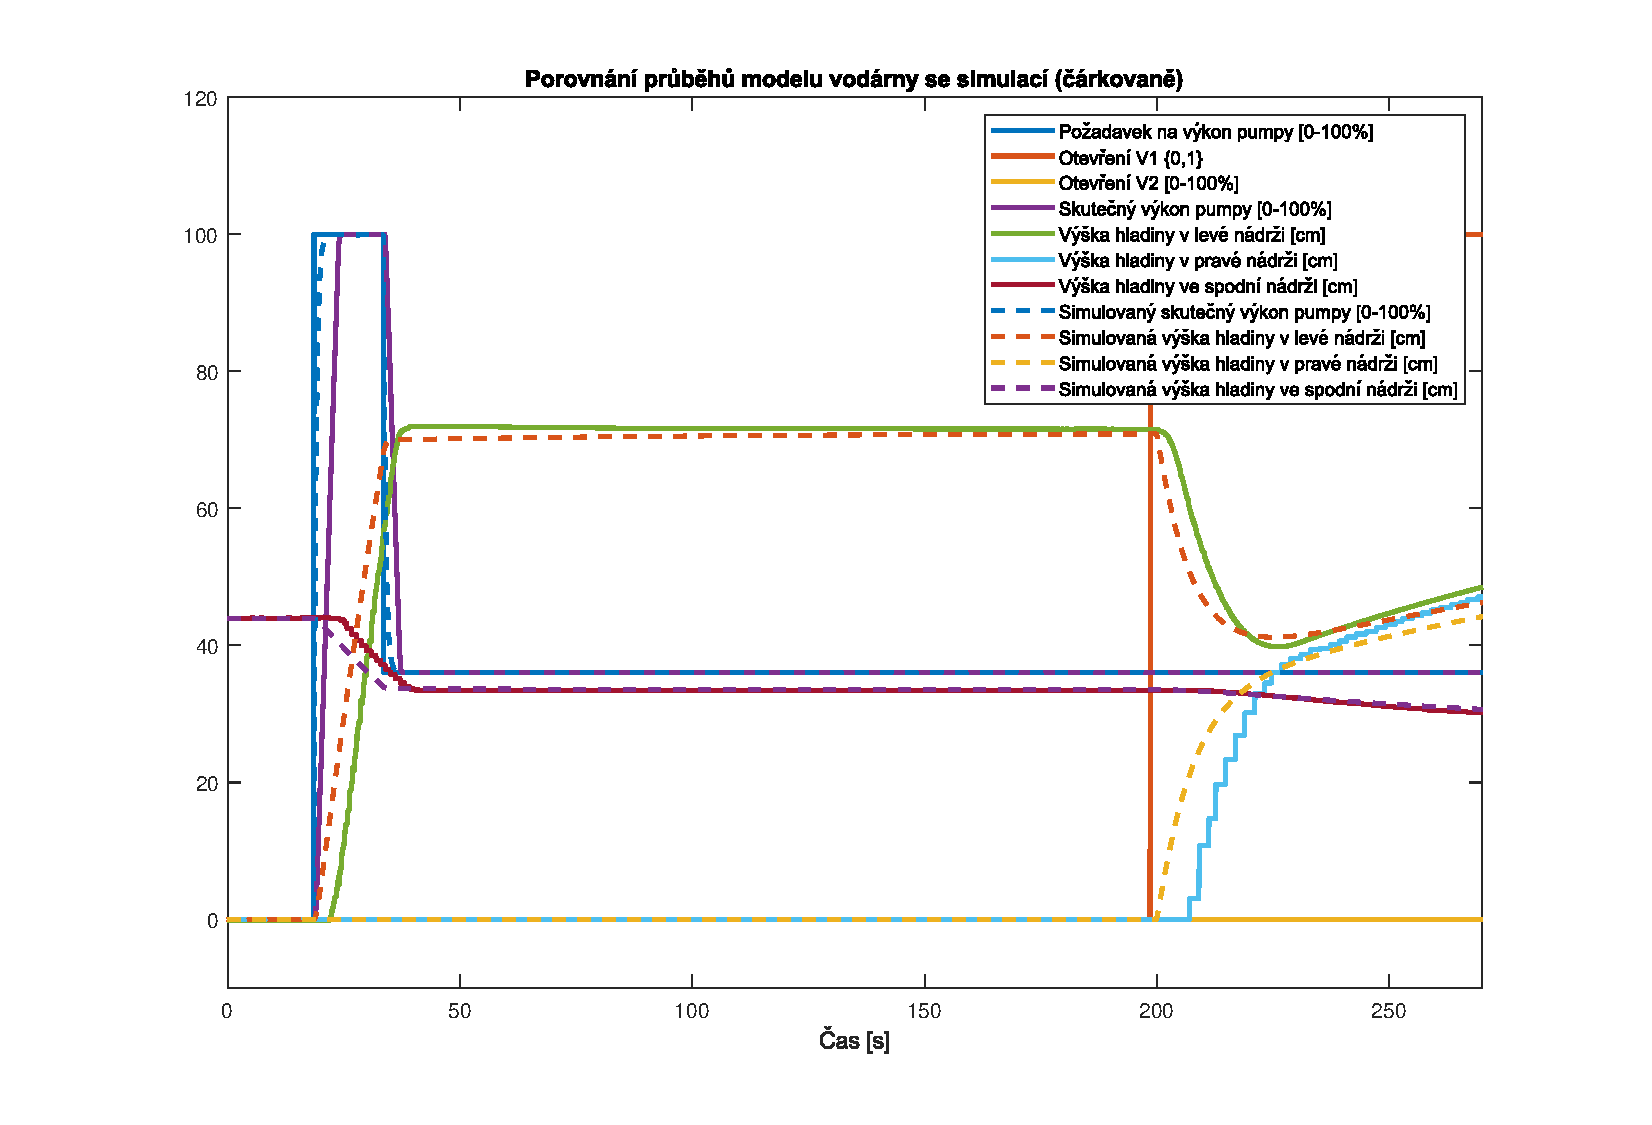
\includegraphics[width=\linewidth]{verifikace_3_start.eps}
    \caption{Verifikace modelu pomocí první části experimentu č. 3}
    \label{fig:verifikace_3_start}
\end{figure}

\begin{figure}[htbp]
    \centering
    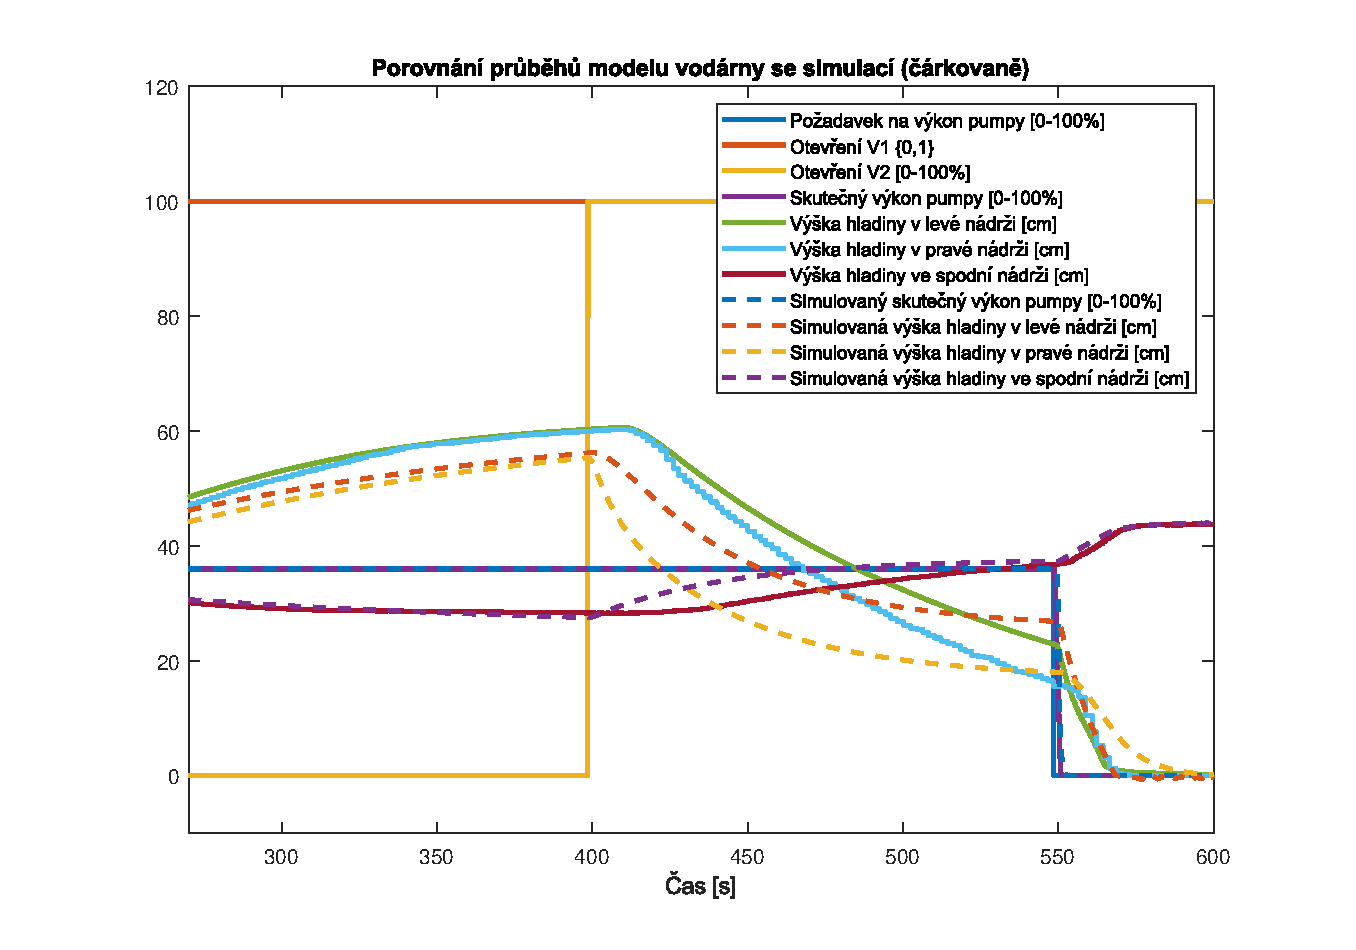
\includegraphics[width=\linewidth]{verifikace_3_end.eps}
    \caption{Verifikace modelu pomocí druhé části experimentu č. 3}
    \label{fig:verifikace_3_end}
\end{figure}

\begin{figure}[htbp]
    \centering
    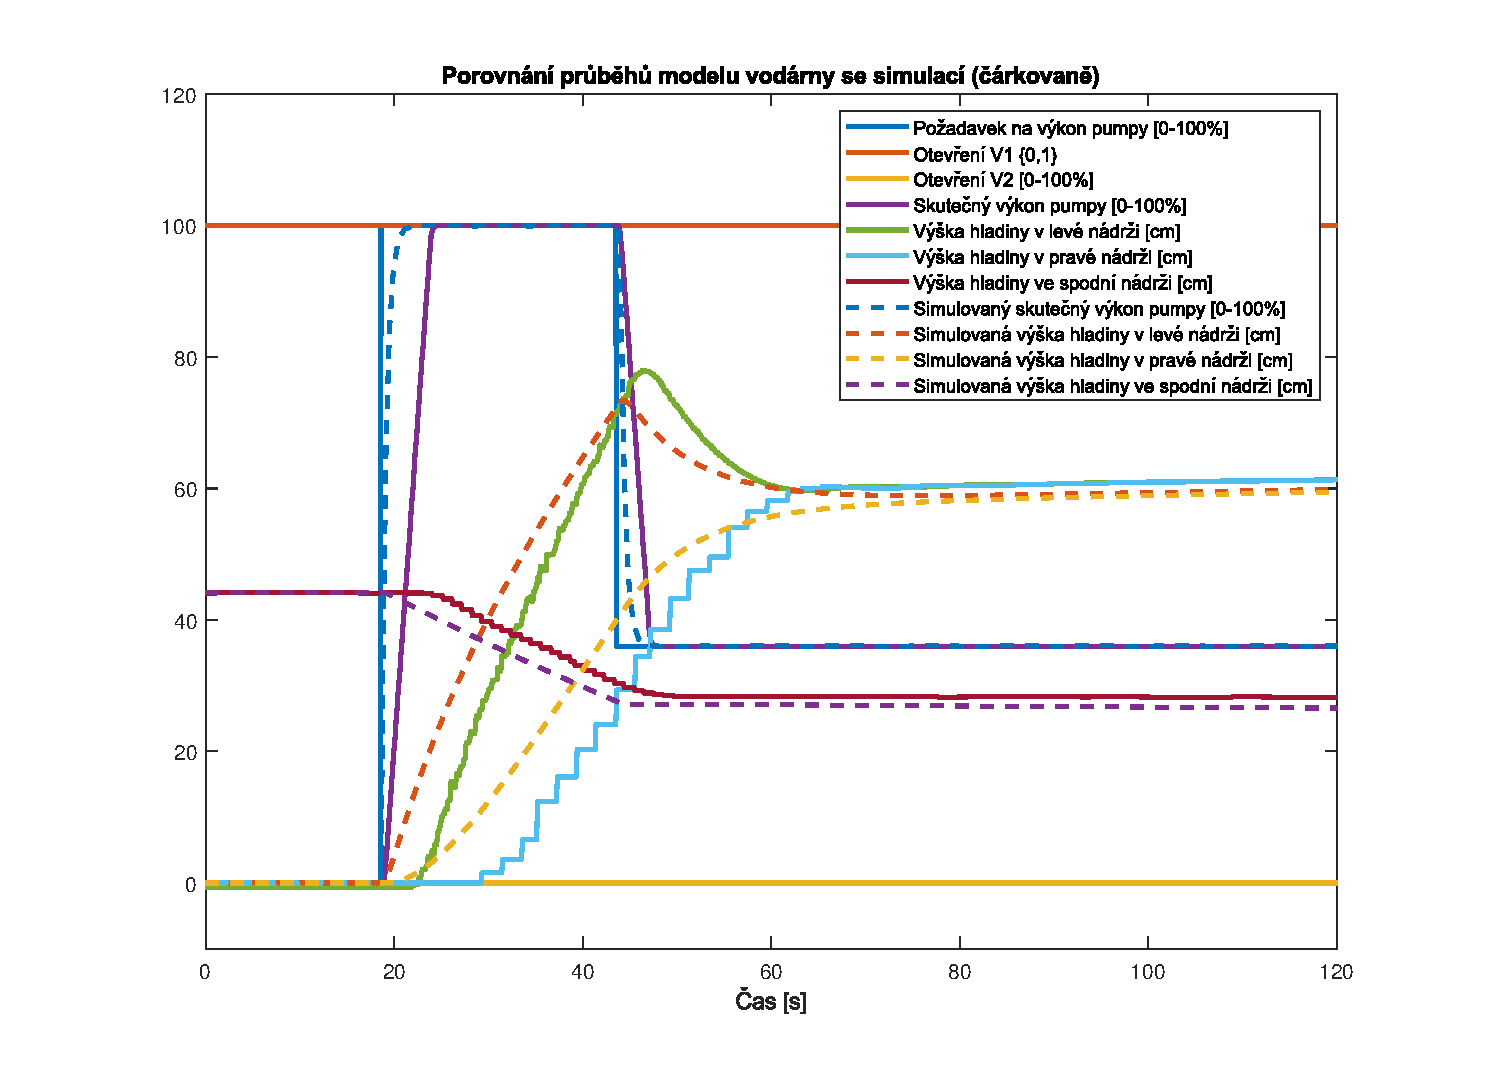
\includegraphics[width=\linewidth]{verifikace_4_start.eps}
    \caption{Verifikace modelu pomocí první části experimentu č. 4}
    \label{fig:verifikace_4_start}
\end{figure}
\begin{figure}[htbp]
    \centering
    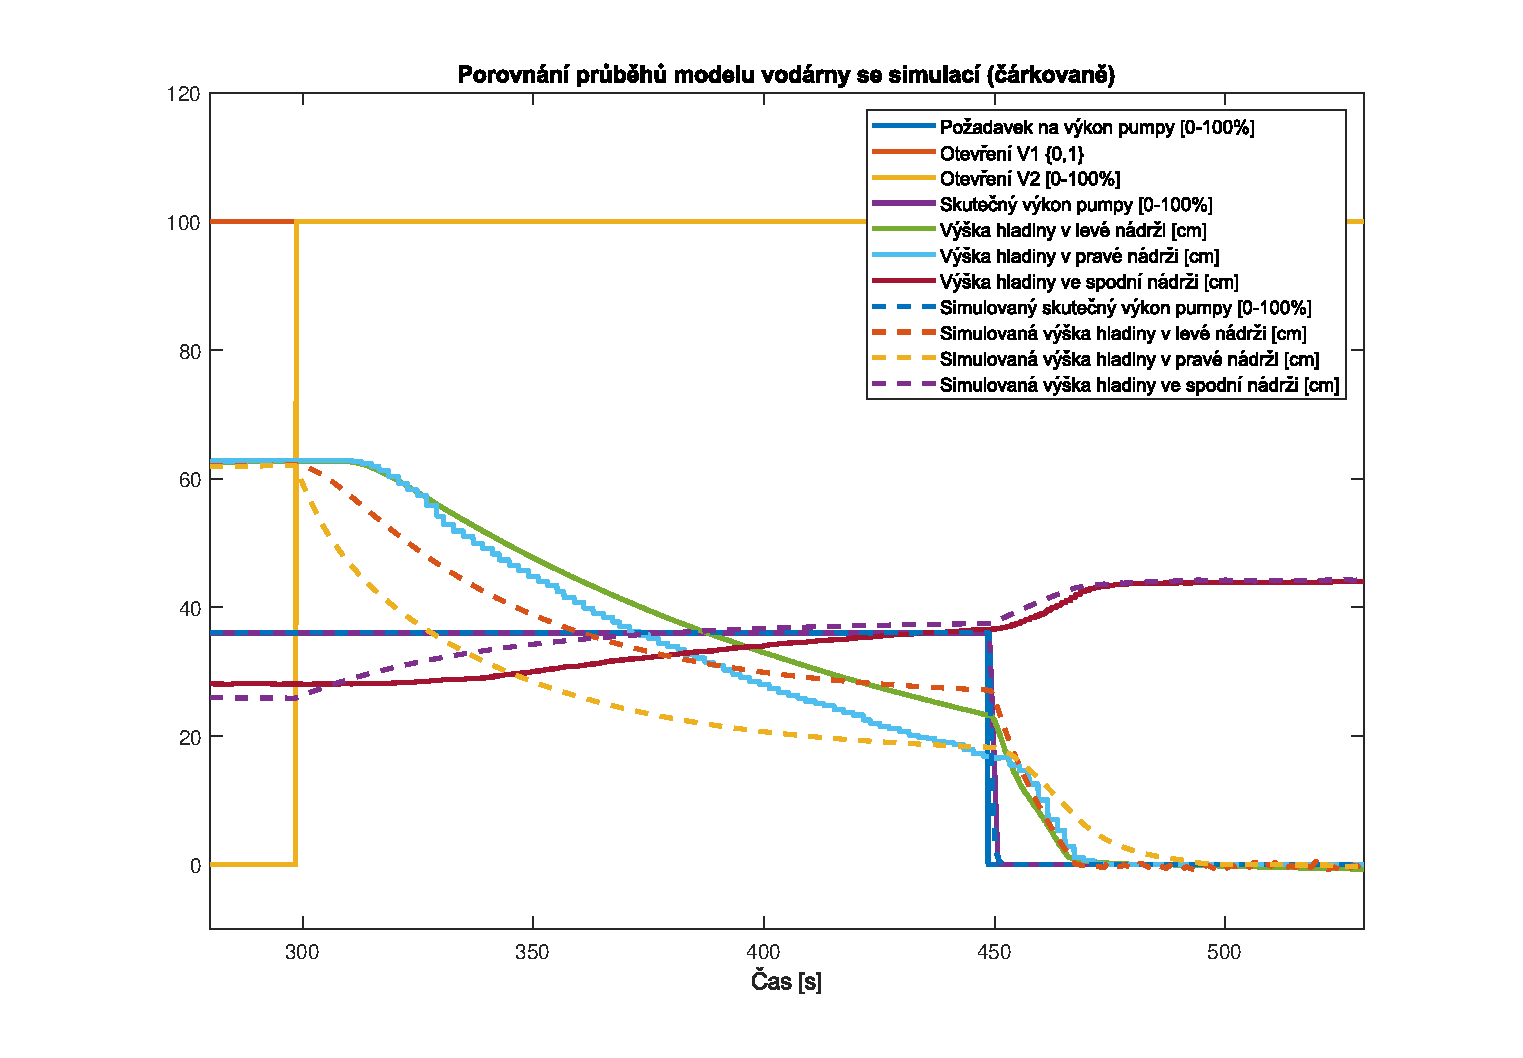
\includegraphics[width=\linewidth]{verifikace_4_end.eps}
    \caption{Verifikace modelu pomocí druhé části experimentu č. 4}
    \label{fig:verifikace_4_end}
\end{figure}

\newpage

\section{Diskuse výsledků}
\label{sec:diskuse}

Vytvořený model má několik zásadních nedostatků:
\begin{itemize}
    \item Čerpadlo ve skutečnosti není lineární systém řádu jedna. Jeho odezva má omezenou rychlost přeběhu
    a~doba ustálení určená během identifikace v sekci \ref{sec:identifikace_cerpadla} má smysl jen pro přeběh z 0 na 35 \% výkonu.
    Pro delší přeběhy (např. z 0 na 100 \%) je z porovnání patrné, že se simulované čerpadlo ustaluje rychleji než reaálné.
    \item Zanedbané dopravní zpoždění ventilů $\text{V}_1$ a~$\text{V}_2$ se výrazně projevuje např. na výstupu simulace \ref{fig:verifikace_4_end}.
    V čase $t\approx 300~\si{\second}$ dojde k~otevření ventilu, ale až o~cca $10~\si{\second}$ později začnou klesat hladiny nádrží $\text{N}_1$, $\text{N}_2$.
    Toto zjednodušení by vnášelo velkou chybu v případě rychlých dějů, na dostupných experimentech však nevyvolalo žádné zásadní problémy.
    \item Modul gyrátoru reprezentující působení čerpadla vycházel odlišně pro každý dataset. Použitá hodnota uvedená v \ref{sec:identifikace_cerpadla}
    se lišila o~$\pm 5~\% (\pm 10~\si{\pascal\per\ampere})$ mezi jednotlivými experimenty a~proto je na všech simulacích patrné nesprávné
    ustálené zesílení systému (hladiny nádrží se ustálí, ale o~pár centimetrů jinde). Toto dle mého názoru není způsobené žádnou
    časovou proměnlivostí čerpadla, spíše to je nepřímý projev nějaké zanedbané dynamiky.
    \item Vypočtená velikost odporu trubek nebyla použitelná pro simulace, protože všechny děje vyrovnávání hladin byly příliš rychlé.
    Pro zpomalení dějů bylo potřeba buď zvětšit odpory, nebo zvětšit moduly poddajností. Moduly poddajnosti (kapacity nádrží)
    jsou však jednoduše určitelné a~odvoditelné, zatímco odpor trubky viskozní kapalině je fyzikální vztah nad mé znalosti.
    Spíše bych proto viděl bychu ve výpočtu odporu. Jednotlivým trubkám bylo potřeba odpor přenásobit konstantou z intervalu $\langle 2, 8 \rangle$,
    aby časové průběhy seděly s~experimenty.

\end{itemize}
Veskrze ale průběhy ze simulací odpovídají průběhům z fyzického modelu. Zjednodušení diskutované v \ref{sec:sloupec_vody} zřejmě nevnáší
do modelu významnou chybu, neboť jsou si dynamika reálné a~simulované nádrže $\text{N}_1$ velmi podobné a~není patrné žádné zpoždění
(způsobené v reálu nutností nejdříve naplnit trubku $\text{T}_1$). 


    
\begin{thebibliography}{9}


    \bibitem{repository}
        Repozitář s~podklady pro úlohu, \url{https://gitlab.fel.cvut.cz/aa4cc/msd/semestralni-ulohy-pro-predmet-msd/-/blob/master/vodarna}
    \bibitem{zadani}
    Zadání semestrální úlohy, \url{https://gitlab.fel.cvut.cz/aa4cc/msd/semestralni-ulohy-pro-predmet-msd/-/blob/master/vodarna/zadani/msd_vodarna.pdf}
    \bibitem{tabulky}
    Fyzikální tabulky, \url{http://kabinet.fyzika.net/studium/tabulky/tabulky.php}

    \bibitem{odpor_trubky}
    Viscosity and Laminar Flow; Poiseuille's Law, Lumen Physics, \url{https://courses.lumenlearning.com/physics/chapter/12-4-viscosity-and-laminar-flow-poiseuilles-law/}
    
    \bibitem{hladinomer}
    Hladinoměr \textbf{Prosonic FMU 40} \url{https://www.cz.endress.com/cs/Polni-instrumentace-sita-na-miru/mereni-hladiny/FMU40?t.tabId=product-overview}

    
    \end{thebibliography}
    

\end{document}

